\chapter{Optimierungen}

In diesem Kapitel wird beschrieben, was für Optimierungen für den Compiler implementiert wurden. Im Forth Cross-Compiler sind schon einige Peephole Optimierungen implementiert. In diesem Kapitel werden die neu implementierten Optimierungen mit dessen des Cross-Compilers verglichen und gezeigt wo noch bessere Optimierungsstrategien verwendet werden können.

\section{Peephole Optimierung}

Peephole Optimierungen ist eine Art von Optimierung, welche auf einer kleinen Sequenz von Instruktionen durchgeführt wird. Dieses Sequenz wird Peephole oder auch Window genannt. Die Peephole Optimierung verucht Sets von Instruktionen durch kürzere oder schnellere Instruktionen zu ersetzen.\cite{peepwiki} Peephole Optimierungen können die grösse der Codes um 15--40 Prozent verkleinern und sind heute in allen gängigen Compilern implementiert.\cite{peepdavidson} Zu der Peephole Optimierung gehören unter anderen folgende Arten von Optimierungen:

\begin{itemize} 
	\item Constant Folding - Konstante Expressions auswerten
	\item Constant Propagation - Konstante Werte in Expressions substituieren
	\item Strength Reduction - Langsame Instruktionen mit äquivalenten schnellen Instruktionen ersetzen.
	\item Combine Operations - Mehrere Oprationen mit einer äquivalenten ersetzen
	\item Null Sequences - Unötige Operationen entfernen\cite{peepwiki}
\end{itemize}

\newpage

\subsection{Beispiele}

Folgend einige Peephole Optimierungs Beispiele anhand von Forth Code.

\subsubsection{Constant Propagation}
\label{constantprogationsection}

Folgende Instruktionen
%
\begin{verbatim}
1
2
swap
+
dup
\end{verbatim}
%
können durch:
%
\begin{verbatim}
2
2
\end{verbatim}
%
ersetzt werden. Die Instruktionen swap, + und dup können schon zur Kompilierzeit durchgeführt werden.
\subsubsection{Combine Operations}
Folgende zwei Instruktionen
%
\begin{verbatim}
rot
rot
\end{verbatim}
%
können durch
%
\begin{verbatim}
-rot
\end{verbatim}
%
ersetzt werden. Die zwei rot Instruktionen sind äquivalent zu einer -rot Instruktion. Oder die folgenden zwei Instruktionen
%
\begin{verbatim}
dup
drop
\end{verbatim}
%
können durch
%
\begin{verbatim}
nop
\end{verbatim}
%
ersetzt werden. Die zwei Instruktionen heben sich auf und können somit entfernt werden.

\newpage

\subsection{Optimierungen}

Für den Compiler wurden Prototypen mässig zwei Optimierungen in Java implementiert. Die erste Optimierung versucht benachbarte Instruktionen zu vereinfachen. Die zweite Optimierung ist eine einfache Constant Propagation. Die beiden Optimierungen werden in den nächsten Kapiteln genauer beschrieben. 

TODO Aktuelle implementation

Der neue Optimizer wird in zwei Phasen durchgeführt:

\begin{figure}[H]
	\centering
		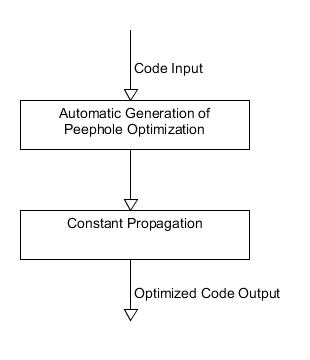
\includegraphics[scale=0.6]{optimizer/optimizer.png}
		\caption{Die zwei Phasen des Optimizers.}
		\captionsetup{margin=0cm,font={footnotesize}}
		\label{fig:extensionpoint}
\end{figure}


Der Peephole Optimizer wird dann 
TODO Optimierungen des Cross-Compilers
TODO Für Projekt zwei Arten implementiert
TODO Ablauf Diagram

\subsection{Automatische Generierung von Peephole Optimierungen}

Klassische Peephole Optimierer versuchen häufig einige Maschinenspezifische Patterns zu korrigieren. Der von Davidson et al. beschriebene Algorithmus (PO) verwendet eine Machine Description und simuliert  benachbarte Instruktionen und versucht diese mit äquivalenten schnelleren Instruktionen zu ersetzen. Für den Forth Optimierer wurde ein Teil des PO objektorientiert implementiert.

\subsection{Constant Propagation}
Unter Constant Propagation versteht man, dass substituieren von Konstanten werden im Code. Dies kann zur Folge haben, dass mehrere Instruktionen schon zur Kompilierzeit ausgewertet werden können wie bei den Beispielen \ref{constantprogationsection} zu sehen ist.

\subsection{Resultate und Tests}
Die Resultate des Optimierers wurden mit verschiedenen Forth Funktionen getestet und die Resultate mit dem Peephole Optimizer des uForth Cross-Compilers verglichen. Die Funktionen sind im Anhang zu finden.

\begin{center}
    \begin{tabular}{ | l | l | l | l | p{8cm} |}
    \hline
    \textbf{Funktion} & \textbf{Orig} & \textbf{Ref} & \textbf{Neu} & \textbf{Kommentar} \\ \hline
    \_Init & 124 & 110 & 116 & Beide Optimizer konnten Code weg optimieren. Die Referenz Implementation konnte vorallem wegen der Regel 3 mehr Instruktionen weg optimieren. Constant Propagation konnte bei der neuen Implementation keine durchgeführt werden.  \\ 
    \hline
    \end{tabular}
\end{center}

Es kann

\subsection{Mögliche Erweiterungen}
SSA
Conditionals und Memory Access
Superoptimizer
in Forth
integrieren in Compiler